%; whizzy chapter
% -initex iniptex -latex platex -format platex -bibtex jbibtex -fmt fmt
% $B0J>e(B whizzytex $B$r;HMQ$9$k>l9g$N@_Dj!#(B


%     Tokyo Debian Meeting resources
%     Copyright (C) 2009 Junichi Uekawa
%     Copyright (C) 2009 Nobuhiro Iwamatsu

%     This program is free software; you can redistribute it and/or modify
%     it under the terms of the GNU General Public License as published by
%     the Free Software Foundation; either version 2 of the License, or
%     (at your option) any later version.

%     This program is distributed in the hope that it will be useful,
%     but WITHOUT ANY WARRANTY; without even the implied warranty of
%     MERCHANTABILITY or FITNESS FOR A PARTICULAR PURPOSE.  See the
%     GNU General Public License for more details.

%     You should have received a copy of the GNU General Public License
%     along with this program; if not, write to the Free Software
%     Foundation, Inc., 51 Franklin St, Fifth Floor, Boston, MA  02110-1301 USA

%  preview (shell-command (concat "evince " (replace-regexp-in-string "tex$" "pdf"(buffer-file-name)) "&"))
% $B2hA|%U%!%$%k$r=hM}$9$k$?$a$K$O(Bebb$B$rMxMQ$7$F(Bboundingbox$B$r:n@.!#(B
%(shell-command "cd image200901; ebb *.png")

%%$B$3$3$+$i%X%C%@3+;O!#(B

\documentclass[mingoth,a4paper]{jsarticle}
\usepackage{monthlyreport}

% $BF|IU$rDj5A$9$k!"Kh7nJQ$o$j$^$9!#(B
\newcommand{\debmtgyear}{2009}
\newcommand{\debmtgmonth}{2}
\newcommand{\debmtgdate}{21}
\newcommand{\debmtgnumber}{49}


\begin{document}

\begin{titlepage}
\thispagestyle{empty}

% $B%?%$%H%k%Z!<%8(B:$BJT=8I,MW$JItJ,$O:G=i$N%^%/%m$KHt$P$9$3$H(B

\vspace*{-2cm}
$BBh(B\debmtgnumber{}$B2s(B $BEl5~%(%j%"(B Debian $BJY6/2q;qNA(B

\hspace*{-2.4cm}
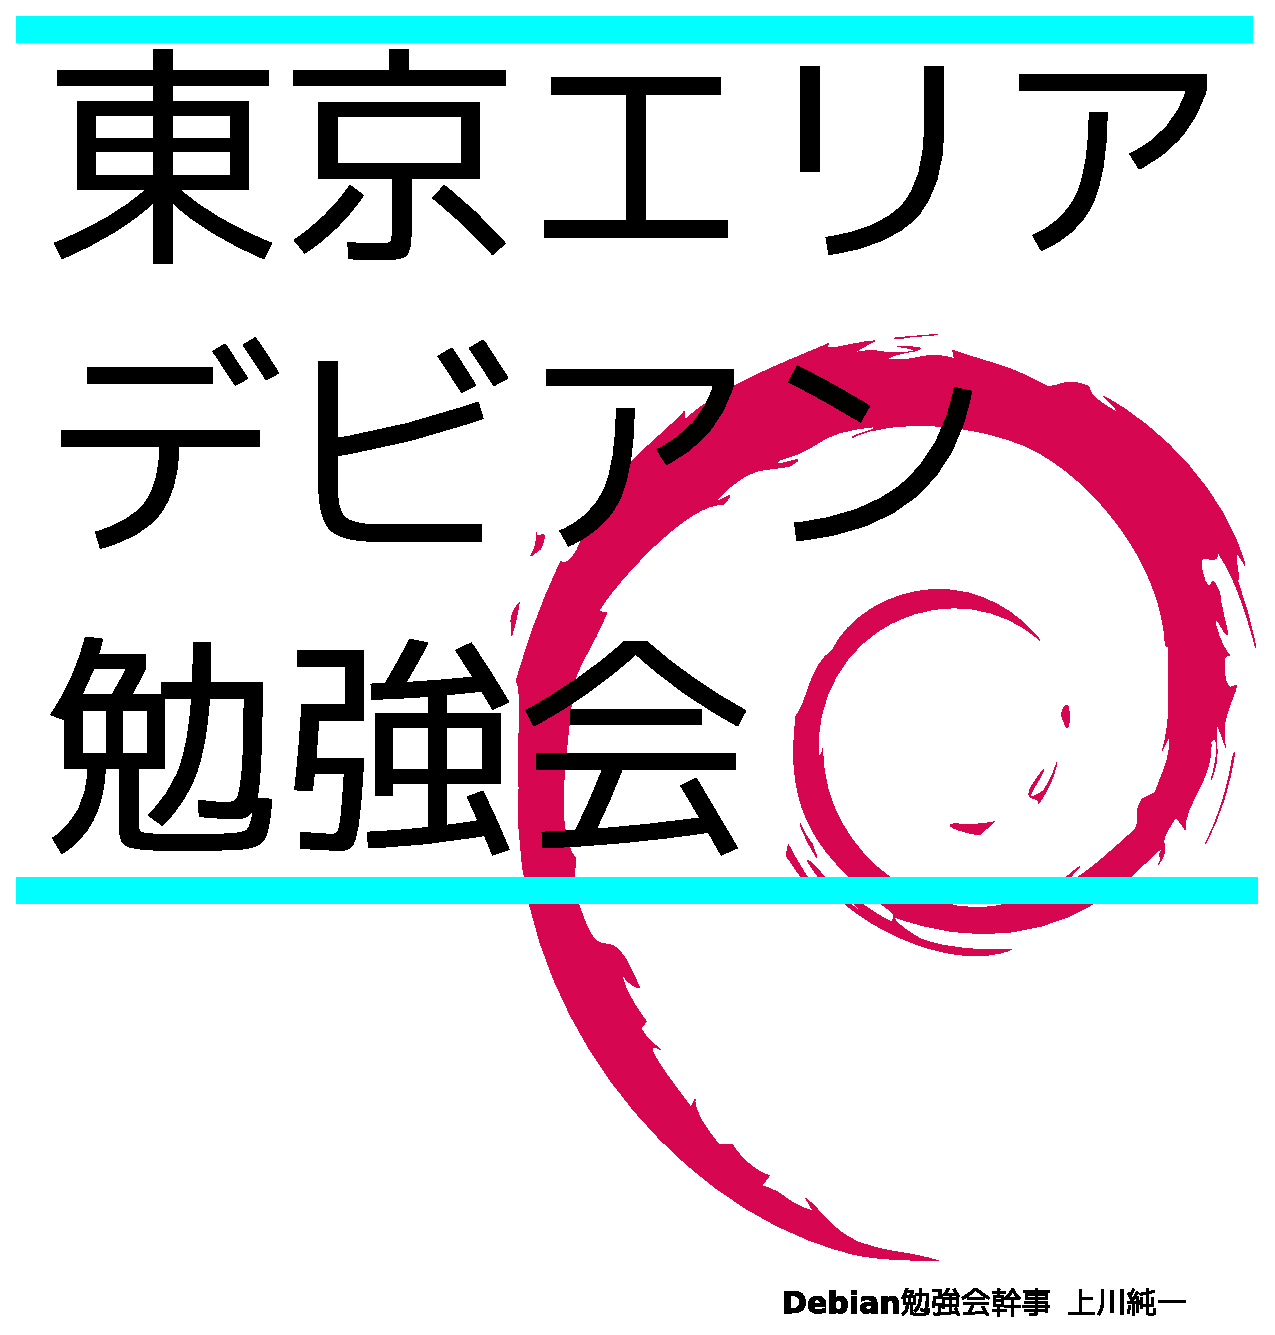
\includegraphics[width=210mm]{image200801/2008title.eps}\\
\hfill{}\debmtgyear{}$BG/(B\debmtgmonth{}$B7n(B\debmtgdate{}$BF|(B

\end{titlepage}

\dancersection{Introduction}{$B>e@n(B $B=c0l(B}

\begin{multicols}{2}
 
 
 $B:#7n$N(BDebian$BJY6/2q$X$h$&$3$=!#$3$l$+$i(BDebian$B$N@$3&$K$"$7$rF'$_F~$l$k$H(B
 $B$$$&J}$b!"$9$G$K$I$C$W$j$H$D$+$C$F$$$k$H$$$&J}$b!"7n$K0l2s(BDebian$B$K$D$$(B
 $B$F8l$j$^$;$s$+!)(B

 Debian$BJY6/2q$NL\E*$O2<5-$G$9!#(B

 \begin{itemize}
 \item \underline{Debian Developer} ($B3+H/<T(B)$B$N0i@.!#(B
 \item $BF|K\8l$G$N!V(B\underline{$B3+H/$K4X$9$k>pJs(B}$B!W$r@0M}$7$F$^$H$a!"%"%C%W%G!<%H$9$k!#(B
 \item \underline{$B>l(B}$B$NDs6!!#(B
 \begin{itemize}
  \item $BIaCJ$P$i$P$i$J>l=j$K$$$k?M!9$,(B face-to-face $B$G=P2q$($k>l$rDs6!(B
	$B$9$k!#(B
  \item Debian $B$N$?$a$K$J$k$3$H$r8l$k>l$rDs6!$9$k!#(B
  \item Debian$B$K$D$$$F8l$k>l$rDs6!$9$k!#(B
 \end{itemize}
 \end{itemize}		

 Debian$B$NJY6/2q$H$$$&$3$H$G5f6KE*$K$O;22C<TA40w$,(BDebian Package$B$r$,$j$,$j(B
 $B$H:n$k%9!<%Q!<%O%C%+!<$K$J$C$?;Q$rLQA[$7$F$$$^$9!#>pJs$N6&M-!&3hMQ$rDL$7(B
 $B$F(B Debian$B$N:#8e$NG=F0E*$JE83+$X$NEZBf$H$7$F!"!V>l!W$H$7$F$N6u4V$rDs6!$9(B
 $B$k$N$,L\E*$G$9!#(B

 2009$BG/$N7W2h$O2>$G$9!#(B

 \begin{enumerate}
  \item $B?7G/$N4k2h(B ($B%"%s%5%s%V%k2.7&3+:E(B)
  \item OSC
  \item ($BEl5~Bg3X(B?)
  \item ($B@iBeED6hETN)?^=q4[(B?\footnote{\url{http://www.library.chiyoda.tokyo.jp/}})
  \item ($BEl5~Bg3X(B?)
  \item 
  \item $B%9%Z%$%s$K$F3+:E(B
  \item Debconf$BJs9p2q(B
  \item 
  \item 
  \item 
  \item $BK:G/2q(B
 \end{enumerate}

 $B2q>l8uJd$H$7$F$O2<5-$,$"$j$^$9(B:

 \begin{itemize}
  \item $BBg3X(B
  \item $B7CHf<w(BSGI$B%[!<%k(B
  \item Google$B%*%U%#%9(B
  \item $B8xL14[(B($B$"$s$5$s$V$k2.7&Ey(B)
  \item $BETN)2q5D<<(B($BL5@~(BLAN)
  \item $B7rJ]$N;\@_(B
 \end{itemize}

\end{multicols}


\newpage

\begin{minipage}[b]{0.2\hsize}
 \definecolor{titleback}{gray}{0.9}
 \colorbox{titleback}{\rotatebox{90}{\fontsize{80}{80} {\gt $B%G%S%"%sJY6/2q(B} }}
\end{minipage}
\begin{minipage}[b]{0.8\hsize}
\hrule
\vspace{2mm}
\hrule
%
% there are too many entries in 200901, usually
% we have tocdepth=2.
%
\setcounter{tocdepth}{1}
\tableofcontents
\vspace{2mm}
\hrule
\end{minipage}



\dancersection{$B:G6a$N(BDebian$B4XO"$N%_!<%F%#%s%0Js9p(B}{$B>e@n(B $B=c0l(B}
\subsection{$BEl5~%(%j%"(BDebian$BJY6/2q(B47$B2sL\Js9p(B}
% (query-replace-regexp "<.*?>" "")
% (query-replace-regexp "^[	 ]\+" "")


\twocolumn
%\dancersection{Debian $B%Q%C%1!<%8%s%0%O%s%:%*%s$N<j0z=q(B}{$B4d>>(B $B?.MN(B}
\section{Debian $B%Q%C%1!<%8%s%0%O%s%:%*%s$N<j0z=q(B}
\subsection{$BK\F|$NL\E*(B}
Debian$B%Q%C%1!<%82=$5$l$F$$$J$$%=%U%H%&%'%"$r%Q%C%1!<%82=$7$F!"(B
$B%S%k%I%F%9%H$H%Q%C%1!<%8$NJQ99$^$G$rBN83$7$^$9!#(B
$B$H$3$m$I$3$m$K%H%i%C%W$,$"$k$N$GCm0U$7$^$7$g$&!#(B
\subsection{$BK\F|$NN.$l(B}
\begin{enumerate}
\item $B9V;U>R2p(B
\item $B:n6H$r;O$a$kA0$NA0=`Hw(B
\item $B%=%U%H%&%'%"$N%3%s%Q%$%k(B
\item $B%Q%C%1!<%8$N?w7A(B
\item CDBS
\item debian$B%G%#%l%/%H%j0J2<%U%!%$%k$NJT=8(B
\item $B%Q%C%1!<%8$N%S%k%I(B
\item $B%Q%C%1!<%8$N%$%s%9%H!<%k(B
\item $B%Q%C%1!<%8$N%S%k%I%F%9%H(B
\item $B%Q%C%1!<%8$N%$%s%9%H!<%k(B/$B%"%s%$%s%9%H!<%k%F%9%H(B
\item $B%W%m%0%i%`$NJT=8(B
\item $B<A5?1~Ez(B
\end{enumerate}


\subsection{$B5-9f$N@bL@(B}
{\bf \$} $B$,IU$$$F$$$k>l9g$O!"%3%s%=!<%k$+$i$NF~NO$r0UL#$7$^$9!#(B{\bf \$}$B$OF~NO$;$:$K(B
$B%3%^%s%I$rF~NO$7$F$/$@$5$$!#(B

$B%3%^%s%I%i%$%s$d%U%!%$%k$NCf?H$G(B{\bf \textbackslash}$B$,=q$+$l$F$$$k>l=j$O9T$,B3$$$F(B
$B$$$k;v$r0UL#$7$^$9!#F~NO$7$J$$$G$/$@$5$$!#(B 

{\bf ...}$B$O>JN,$r0UL#$7$^$9!#<B:]$K$OD9$$=PNO$,$"$k>l9g$K>JN,$7$F$$$k>l(B
$B9g$KMxMQ$7$F$$$^$9!#(B

\subsection{$B%(%G%#%?(B}
$BK\%O%s%:%*%s$G$O!"%(%G%#%?$H$7$F(B{\bf vi}$B$*$h$S(B{\bf mousepad}$B$r;H$($k$h$&$K$7$F$$(B
$B$^$9!#(B{\bf vi}$B$,;H$($J$$?M$O!"(B{\bf mousepad}$B$r;H$C$F$/$@$5$$!#(BWindows$B$N%a%bD"$H(B
$BF1$85!G=$r;}$C$?%(%G%#%?$G$9!#(B

\subsection{$B%k!<%H8"8B$K$D$$$F(B}
$BK\%O%s%:%*%s$G$O!"(Broot$B8"8B$r;H$C$?:n6H$r9T$&>l9g$,$"$j$^$9!#(B
$B$=$N>l9g$K$O(B sudo $B%3%^%s%I$r;H$C$F:n6H$r$7$^$9!#(B{\bf sudo}$B%3%^%s%I$,I,MW$J>l(B
$B9g$K$O%3%^%s%I%i%$%s$N@bL@$N$H$3$m$K(B{\bf sudo}$B$r;XDj$7$F$$$^$9!#(B

\subsection{$BA0=`Hw(B} 
\subsubsection{$B%Q%C%1!<%8%a%s%F%JL>$N@_Dj(B}
$B%Q%C%1!<%8%a%s%F%J$NL>A0$H%a!<%k%"%I%l%9$r4D6-JQ?t$K@_Dj$7$^$9!#(B
$BE,Ev$J$G%(%G%#%?$r;H$C$F!"(B{\bf /home/user/.bashrc} $B$K0J2<$NNc$N$h$&$KJQ(B
$B99$7$FJ]B8$7$F$/$@$5$$!#3F9`L\$K$O<+J,$NL>A0$H%a!<%k%"%I%l%9$r$$$l$F$/$@(B
$B$5$$!#(B
\begin{commandline}
export DEBFULLNAME="Nobuhiro Iwamatsu"
export DEBEMAIL=iwamatsu@nigauri.org
\end{commandline}
$BJ]B8$G$-$?$i!"%?!<%_%J%k$r5/F0$7!"(B
\begin{commandline}
$ source ~/.bashrc
\end{commandline}
$B$r<B9T$7$F$/$@$5$$!#(B

\subsubsection{web$B%5!<%P$NN)$A>e$2(B}
$B%3%s%=!<%k$+$i0J2<$N%3%^%s%I$r<B9T$7$F$/$@$5$$!#$3$l$O(BLive-CD$B4D6-$G(B
apt-get$B$,$G$-$k$h$&$K$9$k$?$a$NBP:v$H$7$F9T$C$F$$$^$9!#<B:]$N%Q%C%1!<%8(B
$B:n@.$G$OI,MW$"$j$^$;$s!#(B
\begin{commandline}
$ sudo ruby1.8 ./tools/web.rb
\end{commandline}

\subsubsection{apt-line$B$NJQ99(B}
$B%(%G%#%?$r;H$$!"(B{\bf /etc/apt/sources.list}$B%U%!%$%k$r0J2<$N$h$&$KJQ99$7$F$/$@$5$$!#(B
apt-line $B$,=q$+$l$F$$$^$9$,!":o=|$7$F$/$@$5$$!#(B
\begin{commandline}
deb http://localhost/debian lenny main
\end{commandline}

\subsubsection{$B%j%]%8%H%j>pJs$N%"%C%W%G!<%H(B}
$B%j%]%8%H%j$N%"%C%W%G!<%H$r9T$$$^$9!#0J2<$N$h$&$K%3%^%s%I$r<B9T$7$^$9!#(B
\begin{commandline}
$ sudo apt-get update
\end{commandline}

\subsubsection{/tmp $B$N%^%&%s%H%*%W%7%g%s$NJQ99(B}
{\bf /tmp}$B$r(B{\bf nodev}$B%*%W%7%g%s$J$7$G(B{\bf remount}$B$7$^$9!#(B
$B0J2<$N$h$&$K<B9T$7$^$9!#(B
\begin{commandline}
sudo mount -o remount,dev /tmp
\end{commandline}

\subsection{$B:#2s$N%5%s%W%k(B}
$B:#2s$O!"(B{\bf cwidget}$B$r;H$C$?%5%s%W%k%W%m%0%i%`(B
{\bf /live/image/osc/data/hello-cwidget-0.1.tar.gz}
$B$rMQ0U$7$^$7$?!#(B
$B$3$N%5%s%W%k%W%m%0%i%`$r(BDebian$B%Q%C%1!<%82=$7$^$9!#(B
{\bf /live/image/osc/data}$B%G%#%l%/%H%j$K%=!<%9%U%!%$%k$,$"$k$N$G!"%[!<%`%G%#%l%/%H%j$KE83+$7$^$9!#(B
\begin{commandline}
$ cd
$ tar -xzf /live/image/osc/data/hello-cwidget-0.1.tar.gz
\end{commandline}

$B$3$N%=%U%H%&%'%"$O(B C++ $B$G5-=R$5$l$F$*$j!"%3%s%Q%$%k$KI,MW$J%i%$%V(B
$B%i%j$d%=%U%H%&%'%"$,%$%s%9%H!<%k$5$l$F$$$k>l9g$K$O!"(B./configure ; make ;
make install $B$G%3%s%Q%$%k$*$h$S%$%s%9%H!<%k$^$G$,$G$-$k$h$&$K$J$C$F$$$^(B
$B$9!#(B

\subsection{$B%Q%C%1!<%8%s%02=3+;O(B}
\subsubsection{$B%=!<%9$rFI$s$G$_$k(B}
$BF0:n$7$J$$%W%m%0%i%`$r%Q%C%1!<(B
$B%82=$7$F$b$7$g$&$,$J$$$N$G!"@h$K$I$N$h$&$J%=%U%H%&%'%"$J$N$+M}2r$9$k$?$a(B
$B$K$b%Q%C%1!<%8%s%02=$9$kA0$K%=!<%9%3!<%I$rFI$s$G!"%=%U%H%&%'%"$NCf?H$rM}(B
$B2r$7$FCV$-$^$7$g$&!#(B

\subsubsection{$B$H$j$"$($:!"%3%s%Q%$%k$7$F$_$k(B}
$BF0$+$J$$%W%m%0%i%`$r%Q%C%1!<%82=$7$F$b$7$g$&$,$J$$$N$G!"F0:n3NG'$r$7$^$9!#(B
$B$^$:$O:GDc8B%3%s%Q%$%k$KI,MW$J%Q%C%1!<%8$r%$%s%9%H!<%k$9$kI,MW(B
$B$,$"$j$^$9!#$=$l$,(B{\bf build-essential}$B%Q%C%1!<%8$G$9!#$3$l$O!"%Q%C%1!<(B
$B%82=$N>l9g$K$bI,MW$G$9!#0J2<$N$h$&$K<B9T$7!"%$%s%9%H!<%k$7$^$9!#(B
\begin{commandline}
$ sudo apt-get install build-essential
\end{commandline}

$B@h$[$I2rE`$7$?%G%#%l%/%H%j$K0\F0$7$^$9!#0\F0$7$?$i!"(B{\bf configure}$B$r<B(B
$B9T$7$^$9!#(B
\begin{commandline}
$ cd hello-cwidget-0.1
$ ./configure
...
Alternatively, you may set the environment variables \
SIGC_CFLAGS
and SIGC_LIBS to avoid the need to call pkg-config.
See the pkg-config man page for more details.
...
\end{commandline}
$B<B9T$9$k$H!"%(%i!<$K$J$j$^$9!#(B
\subsection{$BI,MW$J%i%$%V%i%j$rC5$9(B}
Debian$B$GFCDj$N%U%!%$%k$,Ds6!$5$l$F$$$k%Q%C%1!<%8$rC5$9>l9g$K$O!"(B
{\bf apt-file}$B$rMxMQ$7$^$9!#0J2<$N$h$&$K<B9T$7!"%$%s%9%H!<%k$7$^$9!#(B
\begin{commandline}
$ sudo apt-get install apt-file
\end{commandline}
$BDL>o$O!"(B $B$3$N8e!"(B{\bf apt-file update}$B$r<B9T$7!"%U%!%$%k>pJs%G!<%?$r<hF@$7$^$9$,!"(B
$B4{$K(BLive-CD$B$KF~$l$F$$$k$N$G>JN,$7$^$9!#%U%!%$%k$rC5$9$K$O0J2<$N$h$&$K<B9T$7$^$9!#(B
\begin{commandline}
$ apt-file search pkg-config
...
nant: /usr/share/doc/nant/help/functions/pkg-config.\
     is-max-version.html
pkg-config: /usr/bin/pkg-config
pkg-config: /usr/share/doc/pkg-config/AUTHORS
...
\end{commandline}
$B<B9T$9$k$H!";XDj$7$?%U%!%$%k$rDs6!$7$F$$$k%Q%C%1!<%8L>$,=PNO$5$l$^$9!#(B
$B=PNO$5$l$?%Q%C%1!<%8$r%$%s%9%H!<%k$7$^$9!#(B

\begin{commandline}
$ sudo apt-get install pkg-config
\end{commandline}

$B:FEY(B{\bf configure}$B$r<B9T$7$F$_$^$7$g$&!#(B
\begin{commandline}
$ ./configure
...
No package 'sigc++-2.0' found

Consider adjusting the PKG_CONFIG_PATH environment variable if you
installed software in a non-standard prefix.
...
\end{commandline}
$B$^$@B-$j$J$$%Q%C%1!<%8$,$"$k$h$&$G$9!#@h$[$I$HF1$8$h$&$K(B{\bf apt-file}$B$r(B
$BMxMQ$7$F8!:w$7!"%$%s%9%H!<%k$7$^$9!#(B

\begin{commandline}
$ apt-file search sigc++-2.0.pc
libsigc++-2.0-dev: /usr/lib/pkgconfig/sigc++-2.0.pc
$ sudo apt-get install libsigc++-2.0-dev 
\end{commandline}
$B:FEY(B configure $B$r<B9T$7$^$9!#(B
\begin{commandline}
$ ./configure
...
checking for CWIDGET... configure: error: Package \
  requirements(cwidget) were not met:

No package 'cwidget' found

Consider adjusting the PKG_CONFIG_PATH environment variable \
if you
installed software in a non-standard prefix.
...
\end{commandline}
$B%(%i!<$K$J$j$^$9!#$^$@B-$j$J$$$h$&$J$N$G!":FEY8!:w$7$F%$%s%9%H!<%k$7$^$9!#(B

\begin{commandline}
$ apt-file search cwidget.pc
libcwidget-dev: /usr/lib/pkgconfig/cwidget.pc
$ sudo apt-get install libcwidget-dev
\end{commandline}

\begin{commandline}
./configure
...
config.status: WARNING:  Makefile.in seems to ignore the \
   --datarootdir setting
config.status: creating src/Makefile
config.status: WARNING:  src/Makefile.in seems to ignore the \
  --datarootdir setting
config.status: creating config.h
\end{commandline}

{\bf configure}$B$,@5>o$K=*N;$7$^$7$?!#=*N;$9$k$H!"(B{\bf Makefile}$B$,(B
$B:n@.$5$l$F$$$^$9!#(B{\bf make}$B$r<B9T$7!"%3%s%Q%$%k$7$^$9!#(B
\begin{commandline}
$ make
...
make[1]: $B%G%#%l%/%H%j(B `/home/user/hello-cwidget-0.1' \
$B$KF~$j$^$9(B
Making all in src
make[2]: $B%G%#%l%/%H%j(B `/home/user/hello-cwidget-0.1/src' \
$B$KF~$j$^$9(B
g++ -DHAVE_CONFIG_H -I. -I. -I..     -g -O2 -I/usr/ \
include/sigc++-2.0 \
-I/usr/lib/sigc++-2.0/include   -I/usr/lib/cwidget
 -I/usr/include/sigc++-2.0  -I/usr/lib/sigc++-2.0/include \
 -c hello.cc
g++  -g -O2 -I/usr/include/sigc++-2.0 -I/usr/lib/ \
sigc++-2.0/include   \
-I/usr/lib/cwidget -I/usr/include/sigc++-2.0
-I/usr/lib/sigc++-2.0/include \
-o hello  hello.o  -lsigc-2.0   -lcwidget -lncursesw \
-lsigc-2.0  
make[2]: $B%G%#%l%/%H%j(B `/home/user/hello-cwidget-0.1/src' \
$B$+$i=P$^$9(B
make[2]: $B%G%#%l%/%H%j(B `/home/user/hello-cwidget-0.1' $B$KF~$j$^$9(B
make[2]: $B%G%#%l%/%H%j(B `/home/user/hello-cwidget-0.1' $B$+$i=P$^$9(B
make[1]: $B%G%#%l%/%H%j(B `/home/user/hello-cwidget-0.1' $B$+$i=P$^$9(B
\end{commandline}

$B%3%s%Q%$%k$b@5>o$K=*N;$7$?$N$G!";n$7$K<B9T$7$F$_$^$9!#(B
\begin{commandline}
$ ./src/hello
\end{commandline}

$B$3$3$^$G$O%5%s%W%k%W%m%0%i%`$NF0:n3NG'$G$9!#F0:n$7$J$$%W%m%0%i%`$r%Q%C%1!<(B
$B%82=$7$F$b$7$g$&$,$J$$$N$G!"@h$K$I$N$h$&$J%=%U%H%&%'%"$J$N$+M}2r$9$k$?$a(B
$B$K$b%Q%C%1!<%8%s%02=$9$kA0$K%=!<%9%3!<%IEy$rFI$s$G$*$/$3$H$r$*4+$a$7$^$9!#(B

\subsection{Deban$B%Q%C%1!<%8$N?w7A(B}
{\bf dh\_make}$B%3%^%s%I$G%Q%C%1!<%8$N?w7A$r:n@.$9$k$3$H$,$G$-$^$9!#(B
{\bf dh\_make}$B$O!"(B{\bf dh-make}$B%Q%C%1!<%8$GDs6!$5$l$F$$$^$9!#(B
$B0J2<$N%3%^%s%I$r<B9T$7!"%$%s%9%H!<%k$7$^$9!#(B
\begin{commandline}
$ sudo apt-get install dh-make
\end{commandline}

$B?w7A$N:n@.$O0J2<$N%3%^%s%I$r<B9T$7$^$9!#(B
\begin{commandline}
$ dh_make --createorig -s
\end{commandline}
{\bf --createorig}$B%*%W%7%g%s$O%*%j%8%J%k%=!<%9%3!<%I$N(Btar.gz$B%$%a!<%8$r9=C[$7(B
  $B$^$9!#(B $B:#2s$O%7%s%0%k%P%$%J%j%Q%C%1!<%8!J0l$D$N%=!<%9%3!<%I$+$i0l$D$N(B
  $B%P%$%J%j%Q%C%1!<%8$,:n@.$5$l$k!K$J$N$G(B{\bf -s} $B$r;XDj$7$^$9!#<B9T$9$k$H0J2<(B
  $B$N$h$&$J%a%C%;!<%8$,I=<($5$l$k$N$G!"(BEnter$B%-!<$r2!$7$^$9!#(B
\begin{commandline}
Maintainer name : Nobuhiro Iwamatsu
Email-Address   : iwamatsu@nigauri.org 
Date            : Sun, 15 Feb 2009 23:51:58 +0900
Package Name    : hello-cwidget
Version         : 0.1
License         : blank
Using dpatch    : no
Using quilt     : no
Type of Package : Single
Hit <enter> to confirm: 
\end{commandline}

\subsubsection{debian$B%G%#%l%/%H%j(B}
$B$&$^$/F0:n$9$k$H!"(B{\bf debian$B%G%#%l%/%H%j(B}$B$,:n@.$5$l!"$3$NCf$K?w7A$,:n@.$5$l(B
$B$^$9!#%Q%C%1!<%8%a%s%F%J$O$3$N%G%#%l%/%H%j$NCf0J30$O?($j$^$;$s!#(B
$B0J2<$N$h$&$J>uBV$K$J$C$F$$$^$9!#(B
\begin{commandline}
.
|-- README.Debian  (Debian$B%Q%C%1!<%8$N(B README)
|-- changelog      (Debian$B%Q%C%1!<%8$N%A%'%s%8%m%0(B)
|-- compat         (Debian$B%Q%C%1!<%8$N%P!<%8%g%s(B)
|-- control        (Debian$B%Q%C%1!<%8>pJs(B)
|-- copyright      ($B%3%T!<%i%$%H>pJs(B)
|-- cron.d.ex      (cron $B$r;H$&%Q%C%1!<%8MQ@_Dj%U%!%$%k(B)
|-- dirs           ($B:n@.$9$k%G%#%l%/%H%jL>$r;XDj$9$k(B)
|-- docs           ($B%$%s%9%H!<%k$9$k%I%-%e%a%s%H%U%!%$%k$r;XDj$9$k(B)
|-- emacsen-install.ex (emacs $BMQ@_Dj%U%!%$%k(B)
|-- emacsen-remove.ex  (emacs $BMQ@_Dj%U%!%$%k(B)
|-- emacsen-startup.ex (emacs $BMQ@_Dj%U%!%$%k(B)
|-- hello-cwidget.default.ex (debfonf$BMQ(B)
|-- hello-cwidget.doc-base.EX (doc-base$BMQ(B)
|-- init.d.ex      (init.d$B$r;H$&%Q%C%1!<%8MQ@_Dj%U%!%$%k(B)
|-- init.d.lsb.ex  (init.d$B$r;H$&%Q%C%1!<%8MQ@_Dj%U%!%$%k(B)
|-- manpage.1.ex   (manpage $B$N?w7A(B)
|-- manpage.sgml.ex(manpage $B$N?w7A(B)
|-- manpage.xml.ex (manpage $B$N?w7A(B)
|-- menu.ex        ($B%a%K%e!<$N?w7A(B)
|-- postinst.ex    (postinst$B%a%s%F%J%U%!%$%k$N?w7A(B)
|-- postrm.ex      (postrm$B%a%s%F%J%U%!%$%k$N?w7A(B)
|-- preinst.ex     (preinst$B%a%s%F%J%U%!%$%k$N?w7A(B)
|-- prerm.ex       (prerm$B%a%s%F%J%U%!%$%k$N?w7A(B)
|-- rules          ($B%Q%C%1!<%8%S%k%I%9%/%j%W%H(B)
`-- watch.ex       ($B%"%C%W%9%H%j!<%`%A%'%C%/MQ%U%!%$%k(B)
\end{commandline}

\subsection{CDBS}
./configure ; make ; make install $B$G%Q%C%1!<%8$N%3%s%Q%$%k$,$G$-$k(B
$B%=%U%H%&%'%"$O(B cdbs $B$r;H$C$?J}$,MF0W$K(BDebian$B%Q%C%1!<%82=$G$-$^$9!#(B


\subsubsection{$B0l2s(B hello-cwidget$B%G%#%l%/%H%j$r:o=|$9$k(B}
$B8=>u$G$O@h$[$I$N(B{\bf dh\_make}$B$N7k2L$,;D$C$F$$$k$N$G0l2s!"%5%s%W%k%W%m%0(B
$B%i%`$N%G%#%l%/%H%j$4$H:o=|$7!":FEYE83+$7$^$9!#(B
\begin{commandline}
$ cd 
$ rm -rf hello-cwidget-0.1.*
$ tar -xzf /live/image/osc/data/hello-cwidget-0.1.tar.gz
$ cd hello-cwidget-0.1
\end{commandline}

\subsubsection{dh\_make$B$r<B9T$7!"%Q%C%1!<%8$N?w7A$r:n@.$9$k(B}

{\bf CDBS}$B$r;H$&(BDebian$B%Q%C%1!<%8$N?w7A:n@.$O0J2<$N%3%^%s%I$r<B9T$7$^$9!#(B
\begin{commandline}
$ dh_make --createorig -b
\end{commandline}
{\bf -b}$B%*%W%7%g%s$r;XDj$9$k$H!"(BCDBS $B$r;H$C$??w7A$r:n@.$7$^$9!#(B
$B0J2<$N$h$&$J%a%C%;!<%8$,I=<($5$l$k$N$G!"%(%s%?!<%-!<$r2!$7$^$9!#(B
\begin{commandline}
Maintainer name : Nobuhiro Iwamatsu
Email-Address   : iwamatsu@nigauri.org 
Date            : Sun, 15 Feb 2009 23:51:58 +0900
Package Name    : hello-cwidget
Version         : 0.1
License         : blank
Using dpatch    : no
Using quilt     : no
Type of Package : cdbs
Hit <enter> to confirm: 
\end{commandline}

\subsubsection{$BITMW$J%U%!%$%k$N:o=|(B}
$B:#2s$N%Q%C%1!<%82=$KI,MW$G$O$J$$%U%!%$%k$r(B{\bf debian}$B%G%#%l%/%H%j0J2<$+$i:o=|(B
$B$7$^$9!#(B
\begin{commandline}
$ rm -rf debian/*.ex debian/*.EX
\end{commandline}

\subsubsection{debian/changelog$B%U%!%$%k$NJT=8(B}
{\bf debian/changelog}$B%U%!%$%k$K$O(B{\bf ITP}(Intent To Package)
$B$N%P%0$,4{$K=q$+$l$F$$$k$G:o=|$7$^$9!#0J2<$N$h$&$KJQ99$7$^$9!#(B
\begin{commandline}
hello-cwidget (0.1-1) unstable; urgency=low

  * Initial release.

 -- Nobuhiro Iwamatsu <iwamatsu@nigauri.org> \
                  Wed, 18 Feb 2009 16:31:25 +0000

\end{commandline}
\subsubsection{debian/copyright$B%U%!%$%k$NJT=8(B}
\begin{commandline}
This package was debianized by Nobuhiro Iwamatsu \ 
                                <iwamatsu@nigauri.org> on
Wed, 18 Feb 2009 16:31:25 +0000.

It was downloaded from <http://www.nigauri.org/~iwamatsu/>

Upstream Author:

    Nobuhiro Iwamatsu <iwamatsu@nigauri.org>

Copyright:

    Copyright (C) 2009 Nobuhiro Iwamatsu <iwamatsu@nigauri.org>

License:

    GPLv2

The Debian packaging is (C) 2009, Nobuhiro Iwamatsu \ 
        <iwamatsu@nigauri.org> and
is licensed under the GPL, see `/usr/share/common-licenses/GPL'.
\end{commandline}
\subsubsection{debian/control$B%U%!%$%k$NJT=8(B}
\begin{commandline}
Source: hello-cwidget
Section: devel
Priority: extra
Maintainer: Nobuhiro Iwamatsu <iwamatsu@nigauri.org>
Build-Depends: cdbs, debhelper (>= 7), autotools-dev
Standards-Version: 3.8.0
Homepage: http://www.nigauri.org/~iwamatsu/

Package: hello-cwidget
Architecture: any
Depends: ${shlibs:Depends}, ${misc:Depends}
Description: Debian Packaging Hands-on sample program
 This is sample program of Debian Hands-on done with
 OSC2009 TOKYO Spring.
 This is very easy program that uses CWidget.
\end{commandline}

\subsubsection{$B%Q%C%1!<%8$N%S%k%I(B}

$B%Q%C%1!<%8$N%S%k%I$K$O(B{\bf debuild}$B%3%^%s%I(B $B$r;H$$$^$9!#(B
debuild$B%3%^%s%I$O(B{\bf devscripts}$B%Q%C%1!<%8$GDs6!$5$l$F$$$^$9!#(B
$B$^$?!"$^$@(B {\bf CDBS}$B%Q%C%1!<%8$r%$%s%9%H!<%k$7$F$$$J$$$N$G!"0l=o$K%$%s(B
$B%9%H!<%k$7$^$9!#(B
$B%Q%C%1!<%8$r%$%s%9%H!<%k$7$?$i!"%Q%C%1!<%8$N%S%k%I$r$7$F$_$^$7$g$&!#(B
\begin{commandline}
$ sudo apt-get install devscripts cdbs
$ debuild -us -uc
...
dpkg-buildpackage: full upload (original source is included)
Now running lintian...
W: hello-cwidget: binary-without-manpage usr/bin/hello
W: hello-cwidget: new-package-should-close-itp-bug
Finished running lintian.
\end{commandline}

\subsection{$B%Q%C%1!<%8$N%$%s%9%H!<%k(B}
$B%Q%C%1!<%8$,L5;v%S%k%I$G$-$?$i!"<B:]$K%$%s%9%H!<%k$7$F$_$^$9!#(B
$B%$%s%9%H!<%k$K$O(B dpkg $B%3%^%s%I$r;H$C$F%$%s%9%H!<%k$7$^$9!#%$%s%9%H!<%k$7(B
$B$?$i!"<B:]$KF0$/$+3NG'$7$F$_$^$7$g$&!#(B
\begin{commandline}
$ sudo dpkg -i ../hello-cwidget_0.1-1_i386.deb
$ which hello
$ hello
\end{commandline}

\subsection{$B%Q%C%1!<%8$N%S%k%I%F%9%H(B}
$B%Q%C%1!<%8$,$G$-$?$"$H$K$O%Q%C%1!<%8$N%F%9%H$r9T$$$^$9!#(B
$B%Q%C%1!<%8$N%S%k%I%F%9%H$K$O(B{\bf pbuilder}$B$r;H$$$^$9!#(B
pbuilder$B$O(BDebian$B$KI,MW$J:GDc8B$N4D6-$+$i%S%k%I$r9T$$!"(B
$B0MB84X78Ey$N%A%'%C%/$r9T$C$F%S%k%I%F%9%H$r9T$&%D!<%k$G$9!#(B

\subsubsection{pbuilder$B%Q%C%1!<%8$N%$%s%9%H!<%k(B}
\begin{commandline}
$ sudo apt-get install pbuilder
\end{commandline}

\subsubsection{pbuilder$B4D6-$N9=C[(B}

$B%S%k%I%F%9%H$r9T$&A0$K(Bbase$B%7%9%F%`%$%a!<%8$r9=C[$9$kI,MW$,$"$j$^$9!#(B
$BDL>o$O0J2<$N$h$&$K<B9T$7$^$9$,!"(B
\begin{commandline}
$ sudo pbuilder --create --distribution lenny
\end{commandline}
$B:#2s$O%a%b%j$N@)8B$,$"$k$?$a!"4{$KMQ0U$7$F$"$k(Bbase$B%7%9%F%`%$%a!<%8$rMxMQ(B
$B$7$^$9!#%$%a!<%8$O(B{\bf /live/image/osc/data/base.tgz}$B$K$"$j$^$9!#(B

\subsubsection{$B%Q%C%1!<%8$N%S%k%I%F%9%H(B}

pbuilder $B$G%F%9%H$9$k>l9g$K$O:n@.$5$l$?%Q%C%1!<%8$N(B{\bf dsc}$B%U%!%$%k$r;XDj$7(B
$B$^$9!#$3$N%U%!%$%k$K$O!"(BDebian$B%Q%C%1!<%8$N9=@.$KI,MW$J%U%!%$%kL>$,=q$+$l(B
$B$F$$$k$N$G!"$=$N>pJs$r85$K:F%S%k%I$r9T$&$3$H$,$G$-$^$9!#(B
$B$^$?!"<B9TA0$K(B{\bf apt-get clean}$B%3%^%s%I$r<B9T$7$F%-%c%C%7%e$r%/%j%"$7(B
$B$F$/$@$5$$!#%a%b%j$,B-$j$J$$$?$a$G$9!#(B
\begin{commandline}
$ cd ..
$ sudo apt-get clean
$ sudo pbuilder --build --distribution lenny \ 
     --basetgz /live/image/osc/data/base.tgz \
     --buildplace /tmp hello-cwidget_0.1-1.dsc
...
\end{commandline}

\subsubsection{$B$J$<%(%i!<$K$J$k$N$+(B}
$B@h$[$I$N<j=g$G$d$C$F$b%S%k%I%(%i!<$K$J$j$^$9!#(B
$B$J$<%(%i!<$K$J$k$N$G$7$g$&$+!#9M$($F$_$^$7$g$&!#(B

\subsubsection{$B:F%S%k%I%F%9%H(B}
$B%(%i!<$K$J$kM}M3$O@h$K%$%s%9%H!<%k$7$?%Q%C%1!<%8(B{\bf libcwidget-dev}$B$r%Q%C%1!<(B
$B%8%S%k%I;~$N0MB84X78$r5-=R$9$k%U%#!<%k%I(B{\bf Build-Depends}$B$KDI2C$7$F$$(B
$B$J$$$?$a$G$9!#DI2C$7$F!":F%S%k%I$7$F$_$^$9!#(B
$B:F%S%k%I$K$O0J2<$N$h$&$K<B9T$7$^$9!#:#EY$O$&$^$/%S%k%I$,$G$-$k$O$:$G$9!#(B
\begin{commandline}
$ sudo pdebuild -- --distribution lenny --basetgz \
 /live/image/osc/data/base.tgz --buildplace /tmp
\end{commandline}


\subsection{$B%Q%C%1!<%8$N%$%s%9%H!<%k(B/$B%"%s%$%s%9%H!<%k%F%9%H(B}
$B%Q%C%1!<%8$,%S%k%I$G$-$?$@$1$G$O4n$s$G$O$$$1$^$;$s!#%$%s%9%H!<%k(B/$B%"%s%$(B
$B%s%9%H!<%k$N%F%9%H$b9T$$$^$7$g$&!#(B
$B%Q%C%1!<%8$N%$%s%9%H!<%k(B/$B%"%s%$%s%9%H!<%k$N%F%9%H$K$O(B{\bf piuparts}$B%Q%C(B
$B%1!<%8$r;H$$$^$9!#(B
\subsubsection{piuparts$B$N%$%s%9%H!<%k(B}
$B0J2<$N$h$&$K<B9T$7!"%$%s%9%H!<%k$7$^$9!#(B
\begin{commandline}
$ sudo apt-get install piuparts
\end{commandline}

\subsubsection{$B%Q%C%1!<%8$N%$%s%9%H!<%k(B/$B%"%s%$%s%9%H!<%k%F%9%H(B}
piuparts$B$b(Bpbuilder$B$HF1MM$K:GDc8B$N4D6-$+$i$N%$%s%9%H!<%k$r%A%'%C%/$7$^$9!#(B
$B$h$C$F!"(Bbase$B%7%9%F%`%$%a!<%8$,I,MW$G$9!#IaCJ$O;XDj$9$kI,MW$O$"$j$^$;$s$,!"(B
$B:#2s$O(B{\bf -b}$B%*%W%7%g%s$rIU$1$F!"(B{\bf /live/image/osc/data/base.tgz}$B$K(B
$B$"$k(Bbase$B%7%9%F%`%$%a!<%8$r;XDj$7$F<B9T$7$^$9!#(B
\begin{commandline}
$ cd ..
$ sudo piuparts -d lenny -b /live/image/osc/data/base.tgz \
   hello-cwidget_0.1-1_i386.deb
...
0m41.9s DEBUG: Removed directory tree at /tmp/tmpHliOKO
0m41.9s INFO: PASS: All tests.
0m41.9s INFO: piuparts run ends.
\end{commandline}

\subsection{$B%W%m%0%i%`$NJT=8(B}
hello-cwidget$B$r<B9T$7$F!"0cOB46$N$"$kJ}$,$*$i$l$?$H;W$$$^$9!#(B
$B$=$&!"(B{\bf Lenny}$B$,%j%j!<%9$5$l$?$H$$$&$N$K(B{\bf Etch}$B$K$J$C$F$$$^$7$?!#(B
$B$3$l$O$h$/$J$$$N$GJQ99$7$F$_$^$9!#:#2s$O$h$/MxMQ$5$l$F$$$k(B{\bf dpatch}
$B$r;H$C$F@bL@$7$^$9!#(B
\subsubsection{dpatch$B$N%$%s%9%H!<%k(B}
dpatch$B$r%$%s%9%H!<%k$9$k$K$O!"0J2<$N$h$&$K<B9T$7$^$9!#(B
\begin{commandline}
$ sudo apt-get install dpatch
\end{commandline}
\subsubsection{dpatch$B$r;H$&$?$a$N=`Hw(B}
dpatch$B$r;H$&A0$K!"(B{\bf debian/rules}$B%U%!%$%k$K(Bdpatch$B$r;H$&$h$&$K@_Dj$9$kI,MW$,(B
$B$"$j$^$9!#(Bdpatch$B$O0l2s!"%Q%C%1!<%8$N>uBV$r=i4|2=$7$F$+$i9T$&$?$a$G$9!#(B
{\bf hello-cwidget-0.1} $B%G%#%l%/%H%j$K0\F0$7$F!"(B{\bf debian/rules}$B$r0J2<$N$h$&$K=$@5$7$^$9!#(B

\begin{commandline}
$ cd  hello-cwidget-0.1
\end{commandline}

\begin{commandline}
#!/usr/bin/make -f

include /usr/share/cdbs/1/rules/debhelper.mk
include /usr/share/cdbs/1/class/autotools.mk
include /usr/share/cdbs/1/rules/dpatch.mk
include /usr/share/dpatch/dpatch.make
\end{commandline}

\subsubsection{dpatch$B$N<B9T(B}
dpatch$B$O<+%Q%C%1!<%8$r0l2s%3%T!<$7!"(Bdpatch$B4D6-$K0\9T$7$^$9!#(B
$B$=$NCf$GJQ99$7$F!"(Bdpatch$B4D6-$r=*N;$9$k;~$K:9J,$r:n@.$7$^$9!#(B
dpatch$B4D6-$K0\9T$9$k$K$O(B{\bf dpatch-edit-patch}$B%3%^%s%I$K(B
$B:n@.$9$k:9J,$rJ]B8$9$k%U%!%$%kL>$r;XDj$7$F<B9T$7$^$9!#(B
$B0J2<$N$h$&$K<B9T$7$F$/$@$5$$!#(B
\begin{commandline}
$ dpatch-edit-patch 01_change_dist
\end{commandline}

\subsection{$B%U%!%$%k$NJQ99(B}
$B:#2sJQ99$9$k%U%!%$%k$O(B{\bf src/hello.cc}$B$G$9!#(B
$B%(%G%#%?$r5/F0$7!"BP>]$N%U%!%$%k$rJQ99$7$^$9!#(Bmousepad$B$N>l9g$O0J2<$N$h$&(B
$B$K<B9T$7$^$9!#(B
\begin{commandline}
$ mousepad ./src/hello.cc
\end{commandline}
{\bf Etch}$B$NItJ,$r(B{\bf Lenny}$B$KJQ99$7$?$"$H!"J]B8$7$F%(%G%#%?$r(B
$B=*N;$7$^$9!#(B

\subsubsection{dpatch$B4D6-$r=*N;$9$k(B}
dpatch$B4D6-$r=*N;$9$k$K$O0J2<$N$h$&$K<B9T$7$F$/$@$5$$!#(B
$B<B9T$9$k$H!":9J,$r%U%!%$%k$KJ]B8$7$F(Bdpatch$B4D6-$r=*N;$7$^$9!#(B
\begin{commandline}
$ exit
\end{commandline}

\subsubsection{$B:n@.$5$l$?:9J,(B(patch)$B$NCf?H(B}
$B:n@.$5$l$?:9J,$O(B\\
{\bf debian/patches/01\_change\_dist.dpatch}
$B$H$7$FJ]B8$5$l$F$$$^$9!#0J2<$N$h$&$JFbMF$K$J$C$F$$$k$O$:$G$9!#(B
\begin{commandline}
#! /bin/sh /usr/share/dpatch/dpatch-run
## 01_change_dist.dpatch by Nobuhiro Iwamatsu <iwamatsu@nigauri.org>
##
## All lines beginning with `## DP:' are a description of the patch.
## DP: No description.

@DPATCH@
diff -urNad hello-cwidget-0.1~/src/hello.cc hello-cwidget-0.1/src/hello.cc
--- hello-cwidget-0.1~/src/hello.cc 2009-02-15 06:56:01.000000000 +0000
+++ hello-cwidget-0.1/src/hello.cc  2009-02-18 16:54:40.668274925 +0000
@@ -26,7 +26,7 @@
    toplevel::init();

    widgets::widget_ref dialog =
-       dialogs::ok(L"Hello, Debian GNU/Linux Etch!",
+       dialogs::ok(L"Hello, Debian GNU/Linux Lenny!",
            util::arg(sigc::ptr_fun(toplevel::exitmain)));

    toplevel::settoplevel(dialog);
\end{commandline}
$B%Q%C%A$K$O$J$<$=$N$h$&$J@bL@$r$7$?$N$+!"@bL@$r=q$/I,MW$,$"$j$^$9!#(B
{\bf \#\# DP: No description.}$B$NItJ,$K@bL@$r=q$-$^$9!#(B
$B0J2<$N$h$&$KJQ99$9$k$H$$$$$+$b$7$l$^$;$s!#(B
\begin{commandline}
## DP: Change distributin name from Etch to Lenny.
\end{commandline}

\subsubsection{$B:n@.$7$?:9J,$r%Q%C%1!<%8$KH?1G$5$;$k(B}

$B:9J,$O:n@.$5$l$^$7$?$,!"$3$N$^$^$G$O%Q%C%1!<%8:n@.;~$K:9J,$,E,MQ$5$l(B
$B$^$;$s!#(Bdpatch$B$r;H$C$F:9J,$r%Q%C%1!<%8$KE,MQ$5$;$k$K$O(B{\bf
debian/patches/00list}$B%U%!%$%k$r:n@.$7!"%Q%C%1!<%8$K(B
$B%Q%C%A$r%U%!%$%k$KNs5s$9$kI,MW$,$"$j$^$9!#(B{\bf debian/patches/00list}$B$r(B
$B0J2<$N$h$&$KJQ99$7$^$9!#(B
\begin{commandline}
01_change_dist.dpatch
\end{commandline}

\subsubsection{$B:9J,$rE,MQ$7$?%Q%C%1!<%8$r:n@.$9$k(B}
$B:9J,$rE,MQ$7$?%Q%C%1!<%8$r:n@.$9$k$K$ODL>o$N%Q%C%1!<%8:n@.$HJQ$o$j$^$;$s!#(B
{\bf debuild}$B%3%^%s%I$r;H$C$F:n@.$7$^$9!#(B
\begin{commandline}
$ debuild -us -uc
....
\end{commandline}

\subsubsection{$B%Q%C%1!<%8:n@.%(%i!<$K$J$k(B}
$B@bL@$I$*$j$KA`:n$7$F$$$k?M$O!"%Q%C%1!<%8:n@.%(%i!<$K$J$k$H;W$$$^$9!#(B
$BM}M3$O2?$J$N$+!"9M$($F$_$^$7$g$&!#860x$,J,$+$C$??M$O!":F%S%k%I$7$?8e$K!"<B:]$K(B
$B%$%s%9%H!<%k$7$F!":9J,$,H?1G$5$l$F$$$k$+3NG'$7$F$/$@$5$$!#(B
$B$b$A$m$s(B{\bf pbuilder}/{\bf piuparts}$B$r;H$C$F%Q%C%1!<%8$N%F%9%H$r9T$&;v$bK:$l$:$K!#(B

\subsection{$B<A5?1~Ez(B}
$B0J>e$G!"K\%O%s%:%*%s$O=*N;$G$9!#2?$+<ALdEy$O$"$j$^$9$+!)(B

\cleartooddpage

\vspace*{15cm}
\hrule
\vspace{2mm}
\includegraphics[width=2cm]{image200502/openlogo-nd.eps}
\noindent \Large \bf Debian $BJY6/2q;qNA(B\\ \\
\noindent \normalfont \debmtgyear{}$BG/(B\debmtgmonth{}$B7n(B\debmtgdate{}$BF|(B \hspace{5mm}  $B=iHGBh(B1$B:~H/9T(B\\
\noindent \normalfont $BEl5~%(%j%"(B Debian $BJY6/2q(B $B!JJT=8!&0u:~!&H/9T!K(B\\
\hrule


\end{document}
